\documentclass{article}

\usepackage[english]{babel}
\usepackage[utf8]{inputenc}
\usepackage{amsmath,amssymb}
\usepackage{parskip}
\usepackage{graphicx}
\usepackage{subfigure}
\usepackage{hyperref}
\usepackage{algorithm}
\usepackage{algpseudocode}
\usepackage{multirow}
%\usepackage{algorithmicx}

% Margins
\usepackage[top=2.5cm, left=3cm, right=3cm, bottom=4.0cm]{geometry}

% custom footers and headers
\usepackage{fancyhdr}
\pagestyle{fancy}
\lhead{}
\chead{}
\rhead{}
\lfoot{}
\cfoot{}
\rfoot{Page \thepage}
\renewcommand{\headrulewidth}{0pt}
\renewcommand{\footrulewidth}{0pt}


\usepackage{multicol}
\usepackage{tikz}

% code listing settings
\usepackage{listings}
\usepackage{xcolor}

\definecolor{codegreen}{rgb}{0,0.6,0}
\definecolor{codegray}{rgb}{0.5,0.5,0.5}
\definecolor{codepurple}{rgb}{0.58,0,0.82}
\definecolor{backcolour}{rgb}{0.95,0.95,0.92}
\definecolor{framecolour}{rgb}{0.81,0.81,0.77}

\lstdefinestyle{mystyle}{
    aboveskip={1.0\baselineskip},
    belowskip={1.0\baselineskip},
    backgroundcolor=\color{backcolour},   
    commentstyle=\color{codegreen},
    keywordstyle=\color[rgb]{0.627,0.126,0.941},
    numberstyle=\tiny\color{codegray},
    stringstyle=\color{codepurple},
    basicstyle=\ttfamily\footnotesize,
    %numbers=left,
    frame=single,
    rulecolor=\color{framecolour},
    breakatwhitespace=false,         
    breaklines=true,                 
    captionpos=b,                    
    keepspaces=true,                 
    numbersep=5pt,                  
    showspaces=false,                
    showstringspaces=false,
    showtabs=false,                  
    tabsize=2
}

\lstset{style=mystyle}


%%%%%%%%%%%%%%%%%
%     Title     %
%%%%%%%%%%%%%%%%%
\title{Final report \\ Knowledge distillation for echocardiogram view classification}
\author{
  Andris Freimanis\\
  \texttt{gusandrifr@student.gu.se}
  \and
  Moritz Sprenger\\
  \texttt{gussprmo@student.gu.se}
  \and
  Raouf Bahsoun\\
  \texttt{gusbahsra@student.gu.se}
  \and
  Yu-Ping Hsu\\
  \texttt{gushsuyu@student.gu.se}
}
\date{\today \endgraf\bigskip\vspace*{12cm}
	\textbf{Supervisors}\\
	\centering Yinan Yu, academic supervisor, yinan@chalmers.se \\
	Charlotte von Numers, industry supervisor, charlotte.vonnumers@astrazeneca.com \\
	Luis Arevalo, industry supervisor, imarevost@gmail.com}



\begin{document}
\maketitle

%%%%%%%%%%%%%%%%%
%   Problem 1   %
%%%%%%%%%%%%%%%%%
\newpage
\tableofcontents
\newpage
\section{Introduction}
In recent years deep neural networks (DNNs) have become the state-of-the-art in many application domains such as computer vision, natural language processing or game playing using reinforcement learning. These advances can partly be attributed to the availability of more specialized computing power enabling larger models with millions or, especially in the case of large language models, billions of parameters. Training or using these models therefore requires the usage of cloud services or large amounts of storage and computing resources.

With the widespread use of mobile and edge devices in every day life and commercial contexts it is natural to leverage the abilities of DNNs on these devices for a multitude of use cases such as language translation or image classification. With some applications having strict latency, privacy or connectivity requirements, preventing the usage of cloud-based services, it becomes infeasible to use such large models because of memory, computational and energy consumption limitations. This makes it critical to develop methods that are aimed at reducing size and/or inference time of models while keeping a similar performance.

This work gives an overview over the three most used compression techniques for DNNs: pruning, quantization and knowledge distillation. Due to the limited scope and length of this work, the presented approaches only represent a small fraction of the published literature and should mainly serve as an introduction to the field, stressing the main concepts for different distillation techniques.
\newpage
\section{Literature Review}
A cornerstone of model compression, knowledge distillation, remains a central focus of this exploration. Li et al. recent work on “Curriculum Temperature for Knowledge Distillation” is an innovative contribution to this field \cite{li2023curriculum}. The article presents the concept of curriculum temperature adaptation, which enables dynamic control over the temperature parameter in knowledge distillation. This dynamic adaptability offers student models not only to gather knowledge from teachers but also adapt to evolving data distributions. This innovative approach has helped make knowledge distillation more adaptive, dynamic, and efficient.

In addition, “Conditional Teacher-Student Learning” by Meng et al. has broadened the perspective of knowledge distillation \cite{meng2019conditional}. Their method introduces a dynamic teacher selection mechanism that tailors the choice of teacher models to the characteristics of input data. This adaptation ensures that the student network can choose from a selection of teacher models, each suited to specific input conditions. This approach promises substantial gains in both efficiency and accuracy, potentially setting the stage for customizing knowledge distillation techniques to real-world data scenarios.

“Learning Efficient Object Detection Models with Knowledge Distillation” by Chen et al. provides an overview of knowledge distillation techniques, highlighting its significance in model compression \cite{chenLearningEfficientObject2017}. The article provides an understanding of the principles and methods employed in knowledge distillation, making ground for the approaches presented by Li et al. \cite{li2023curriculum} and Meng et al. \cite{meng2019conditional}. Meanwhile, the article by Hinton et al. “Distilling the Knowledge in a Neural Network” laid the groundwork for knowledge distillation, introducing the concept of teacher-student model learning and its potential to improve model generalization \cite{hintonDistillingKnowledgeNeural2015}.

Further exploring the literature, “A Survey of Quantization Methods for Efficient Neural Network Inference” by Gholami et al. is an important resource in terms of model compression \cite{gholamiSurveyQuantizationMethods2021}. This survey presents various quantization techniques, highlighting the potential for significant compression with minimal accuracy loss. The survey by Choudhary et al., “A comprehensive survey on model compression and acceleration”, introduces additional importance to these techniques in the context of resource-constrained deployments \cite{choudharyComprehensiveSurveyModel2020}.
\newpage
\section{Methods/Prerequisites}
Given the described initial conditions for our project, we decided to focus on offline response-based knowledge distillation techniques and investigate the trade-off between performance and model size/speed. This can be explained by the availability of an already trained and well performing teacher network and the transferability of response-based implementations between different network structures.

Following the conducted literature review we identified three response-based knowledge distillation techniques suitable for the required task.
Following \cite{hintonDistillingKnowledgeNeural2015} the knowledge of a network can be distilled by matching the \textit{logits} and in the case of (multi-class) classification the softmax distribution of the teacher and student networks. The distillation loss $ L_D $ can then be expressed as in equation \ref{eq:dist_loss}, where $ L(.) $ is a loss function and $ p(.) $ the softmax function and $ z_t, z_s $ the logits for teacher and student respectively \cite{gouKnowledgeDistillationSurvey2021}.
\begin{equation}
\label{eq:dist_loss}
L_D = L(p(z_t), p(z_s))
\end{equation}
Hinton et al. argue that richer information about similarities between samples and thus more knowledge is transferred between teacher and student, when soft targets are used. They adapt the softmax function by using a scaling parameter $ T $, the temperature, to increase the entropy of the resulting probability distribution. Equation \ref{eq:softmax_T} shows this adapted softmax function with $ z_i $ as the logit for class $ i $ and $ T $ as the temperature \cite{hintonDistillingKnowledgeNeural2015}.

\begin{equation}
\label{eq:softmax_T}
p(z_i, T) = \frac{exp(z_i / T)}{\sum_{j}exp(z_j/ T)}
\end{equation}
Combining equations \ref{eq:dist_loss} and \ref{eq:softmax_T} leads to equation \ref{eq:dist_loss_final}, the distillation loss with soft targets where $ L_{KL} $ is the Kullback Leibler divergence loss.
\begin{equation}
\label{eq:dist_loss_final}
L_D(p(z_t, T), p(z_s, T)) = L_{KL}(p(z_t, T), p(z_s, T))
\end{equation}
To make use of the information in the training data, the student is trained with, the distillation loss is usually combined with the student loss $ L_S $, which is the cross-entropy loss between student outputs and the ground truth labels $ L_S = L_CE(y, p(z_s, T=1)) $. In combining these two losses, we arrive at the joint loss given in equation \ref{eq:joint_loss}, where $ \alpha $ is a balancing parameter between the two losses and the multiplication with $ T^2 $ is done to normalize the magnitude of the gradients \cite{hintonDistillingKnowledgeNeural2015}. Training with this loss function as an objective is further referred to as vanilla knowledge distillation.
\begin{equation}
\label{eq:joint_loss}
L_J = \alpha  (L_D * T^2) + (1 - \alpha) L_S
\end{equation}


Meng et al. observe that it can improve results to only use the distillation loss when the teacher network makes a correct prediction and name this approach conditional teacher student learning \cite{meng2019conditional}. This simplifies the joint loss $ L_J $ by only using the distillation loss with soft labels replaced by the one-hot encoded hard labels for samples where the teacher network makes an incorrect prediction. Thereby, the heuristic tuning of hyperparameter $ \alpha $ can be avoided.

Both introduced methods so far make use of a static heuristically chosen hyperparameter $ T $ for the knowledge distillation. Zheng et al. argue that a dynamic temperature $ T $, would benefit the distillation process inspired by curriculum learning, where the learning difficulty is increased through the training process \cite{liCurriculumTemperatureKnowledge2022}. The dynamic temperature is modeled as a temperature module that gets learned in an adversarial manner. The temperature module is optimized in the opposite direction of the student, trying to maximize the distillation loss with the update shown in equation \ref{eq:temp_gradient} \cite{liCurriculumTemperatureKnowledge2022}.

\begin{equation}
\label{eq:temp_gradient}
\theta_{temp} = \theta_{temp} + \mu \frac{\partial L}{\partial \theta_{temp}}
\end{equation}
To adopt the curriculum learning and change the difficulty of the task throughout the training, the loss w.r.t. the temperature is scaled by $ \lambda $, leading to equation \ref{eq:scaled_temp_gradient} \cite{liCurriculumTemperatureKnowledge2022}.
\begin{equation}
\label{eq:scaled_temp_gradient}
\theta_{temp} = \theta_{temp} + \mu \frac{\partial(\lambda L)}{\partial \theta_{temp}}
\end{equation}
$ \lambda $ increases with each epoch $ E_n $ during the training according to either a linear schedule or a cosine schedule given in equation \ref{eq:cos_schedule}, where $  \lambda_{min} $ and $  \lambda_{max} $ are the range for $ \lambda $ and $ E_{cap} $ is the epoch at which $ \lambda $ reaches it maximum and stays constant. The linear schedule also adopts the same methodology with $ E_{cap} $.
\begin{equation}
\label{eq:cos_schedule}
\lambda_{n} = \lambda_{min} + \frac{1}{2}(\lambda_{max}-\lambda_{min})(1 + cos((1+\frac{min(E_n, E_{cap})}{E_{cap}})\pi))
\end{equation}
Adopting their implementation of a global temperature, $ T $ is a single learnable parameter used for each sample in a batch before being updated with its gradient \cite{liCurriculumTemperatureKnowledge2022}. Following Zheng et al. we set $  \lambda_{min} $ and $  \lambda_{max} $ at $ 0 $ and $ 1 $ as well as $ E_{cap} $ at $ 10 $ as our default values.

\section{Experimental setup}
In accordance with the project goals an ablation study with $ 4 $ different student architectures and the $ 3 $ described distillation techniques is conducted. As for student architectures we focused on efficient convolutional architectures especially designed for mobile and edge devices. The four considered architectures are \textit{Mobilenet-V3-small}, \textit{Mobilenet-V3-large} \cite{mobilenetv3}, Shufflenet \cite{shufflenet} and Ghostnet \cite{han2020ghostnet}. All network implementations are taken from PyTorch \cite{pytorch}. To confirm with the expected input sizes of these architectures, the greyscale image data is duplicated along the channel axis. Additionally, images are resized to $ 112 $\textit{px} sized square images and normalized. Throughout all experiments a batch size of $ 256 $ is used and models are trained for $ 20 $ epochs with early stopping. For all $ 4 $ student architectures experiments are performed with the $ 3 $ different knowledge distillation techniques and training from scratch without any distillation. For vanilla knowledge distillation different values for the temperature are investigated. Conditional knowledge distillation is conducted with a temperature of $ 4 $. For the curriculum-based knowledge distillation linear and cosine decay are investigated.
As performance metrics we report validation accuracy and validation $ F1 $-score. For size and speed metrics, the inference and train speed are reported as well as the model size in \textit{Megabytes} and the number  of trainable parameters.
All experiments are conducted with a single \textit{Nvidia A40} GPU. 

\section{Results}

\begin{figure}
	\centering
	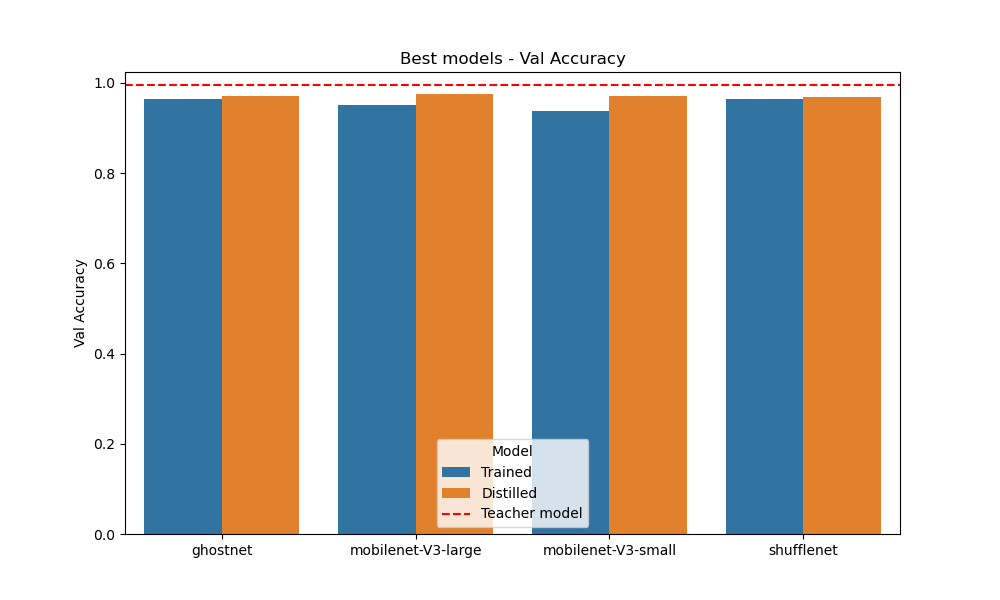
\includegraphics[width=\linewidth]{assets/val accuracy_Best}
	\caption{Results for different student architectures}
	\label{fig:acc_res}
\end{figure}

\begin{figure}
	\centering
	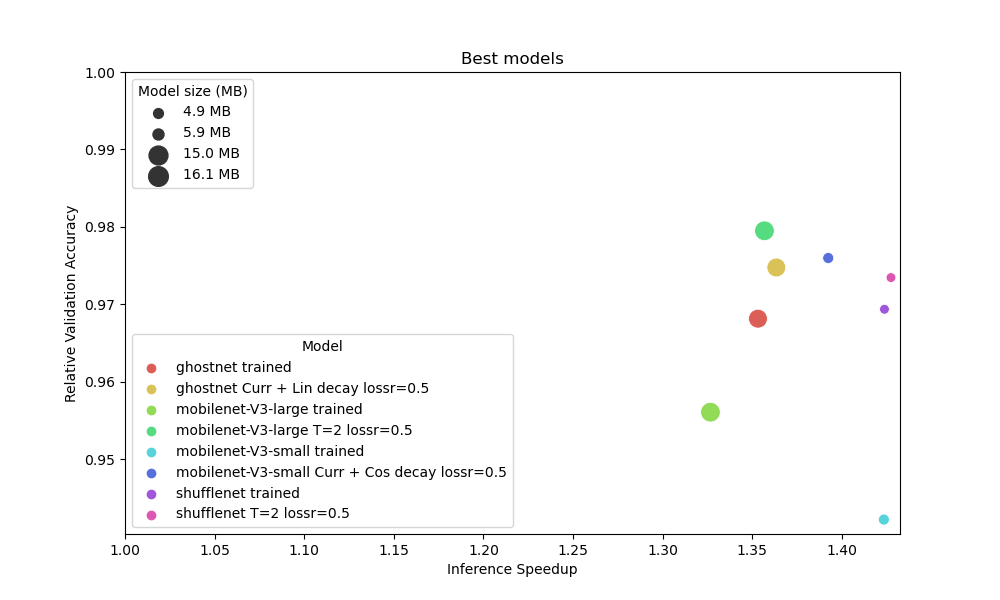
\includegraphics[width=\linewidth]{assets/fat_plot_best}
	\caption{Results for different student architectures}
	\label{fig:scatter_res}
\end{figure}

\begin{figure}
	\centering
	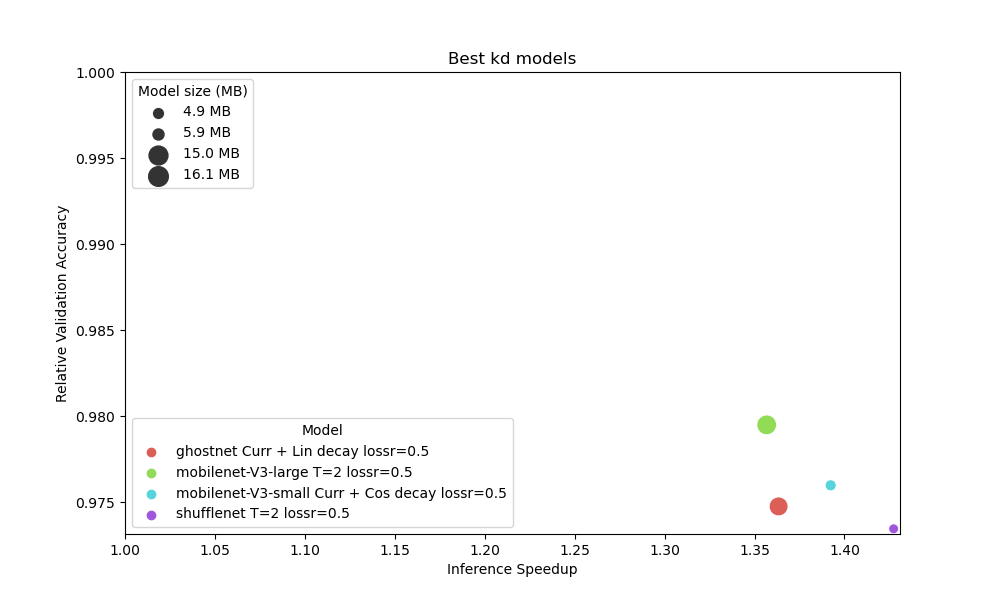
\includegraphics[width=\linewidth]{assets/fat_plot_best KD}
	\caption{Results for different student architectures}
	\label{fig:scatter_kd_res}
\end{figure}

% Our experiments yielded promising results, demonstrating the effectiveness of knowledge distillation for Convolutional Neural Networks (CNNs). We present our findings in two plots.

In Figure \ref{fig:acc_res}, the validation accuracy of the teacher model is represented by a red dashed line, while the best Knowledge Distillation (KD) model and the model trained from scratch for each of the four student architectures are also plotted. It's interesting to note that the validation accuracies of the KD models are not only closely aligned with that of the teacher model, indicating successful knowledge transfer, but they also marginally yet consistently outperform the models trained from scratch for each student architecture. This suggests that all architectures perform comparably well and that KD provides a slight but consistent advantage. The validation accuracy is very close to the teacher for all student architectures.

In our experiments, each student architecture had a different set of optimal hyperparameters. The GhostNet model achieved its best performance using curriculum learning with a linear decay schedule for temperature and a loss rate of 0.5. For the MobileNet V3 Large and ShuffleNet models, the optimal performance is obtained with a temperature parameter of 2 and a loss rate of 0.5. On the other hand, the MobileNet V3 Small model performs best when curriculum learning is combined with cosine decay schedule for temperature and a loss rate of 0.5.

In Figure \ref{fig:scatter_res}, a scatter plot is presented that illustrates the relative validation accuracy (compared to the teacher model) and inference speedup of each student model, both for models trained using Knowledge Distillation (KD) and those trained from scratch. The thickness of each point represents the memory footprint of the model in MB.

All KD student models achieved similar performance, with relative validation accuracies ranging from 0.975 to 0.98 and inference speedups between 1.35 and 1.4 times. However, the models trained from scratch showed a decrease in accuracy down to 0.95. This reinforces the effectiveness of KD, as it consistently outperforms training from scratch.

Interestingly, there are some variations in the inference speed even between models with the same architecture. This could be attributed to slightly inconsistent allocation of hardware resources and memory index management. Despite these variations, the inference speed is generally close for all architectures.

Among all models, MobileNet V3 Large had the highest relative validation accuracy at 0.98. The two smaller models, MobileNet V3 Small and ShuffleNet, achieved slightly higher inference speedups of 1.4 times.

These results suggest that KD enables student models to achieve comparable performance to their teacher models while benefiting from increased inference speed and reduced memory usage.

Figure \ref{fig:scatter_kd_res} provides a focused view on only the KD models, further emphasizing these observations.

\section{Limitations}
Due to the limited available time for the project and project specific circumstances multiple limitations have to be considered regarding the achieved results. Because of significant training times and the time constraints set by the project course the search space for different hyperparameter combinations was heavily restricted. With the same reasoning no statistical significance testing was performed and experiments for each setup only performed once. This weighs even more heavy for this project since the student model reach very good results even without knowledge distillation and the different distillation techniques are very close in performance. Therefore, the results can only be interpreted as indications, especially regarding the differences between different knowledge distillation techniques.
For a few experiments a batch size of $ 32 $ was also tested and achieved slightly better results but due to the increased training time with a reduced batch size, this was not further pursued.
The captured data for training and inference speed is very noisy likely because of the shared nature of the computing resource, therefore for speeds the median batch time or the minimum epoch times are reported.

\newpage
"The computations/data handling/[SIMILAR] were/was enabled by resources provided by the National Academic Infrastructure for Supercomputing in Sweden (NAISS) at [NAISS AFFILIATED SITE] partially funded by the Swedish Research Council through grant agreement no. 2022-06725."
\section*{Appendix}
\bibliographystyle{plain}
\bibliography{bib}

\end{document}

